\documentclass[11pt,a4paper]{article} 
\usepackage[T1]{fontenc}
\usepackage[utf8]{inputenc}
\usepackage{lmodern}
\usepackage[a4paper,margin=2.5cm]{geometry}
\usepackage{graphicx}
\usepackage{booktabs}
\usepackage{longtable}
\usepackage{array}
\usepackage{float}
\usepackage{listings}
\usepackage{xcolor}
\usepackage{hyperref}
\usepackage{enumitem}

\lstset{   
basicstyle=\ttfamily\small,   
breaklines=true,   
frame=single,   
numbers=left,   
numberstyle=\tiny\color{gray},   
keywordstyle=\color{blue},   
commentstyle=\color{green!50!black},   
stringstyle=\color{red!60!black},   
backgroundcolor=\color{gray!5}, 
}

\title{Comparative Evaluation of Static Analysis Tools\\
on Original and Mutated Test Cases }

\author{Pomsár Jakub\\   
Faculty of Informatics\\   
Masaryk University\\
582923@mail.muni.cz }
\date{\today}

\begin{document}

\maketitle

\begin{abstract} This report presents a comparative evaluation of three static analysis tools: Cppcheck, Clang Static Analyzer, and Facebook Infer. The tools are compared on selected test cases from the NIST Juliet Test Suite for C/C++ and on modified variants generated through systematic source-level transformations. The goal is to investigate differences in detection capability, analysis runtime, and behavioral characteristics across tools that embody fundamentally different static analysis paradigms: pattern-based checking, inter-procedural symbolic execution, and abstract interpretation with bi-abduction. The vulnerability categories under study are memory leaks (CWE-401), double free (CWE-415), use-after-free (CWE-416), uninitialized variables (CWE-457), and null pointer dereferences (CWE-476).
\end{abstract}

\tableofcontents
\newpage

\section{Introduction} 
\subsection{Motivation}

Static analysis is one of the widely used techniques in modern software development pipelines to detect bugs and security vulnerabilities before code ever executes. Unlike dynamic testing, a static analyzer operates on source or intermediate representations directly and can reason about execution paths that may not be exercised by a particular test suite.

The C and C++ languages remain dominant in systems programming, embedded development, and performance-critical applications, yet they expose programmers to a class of memory-safety errors (use-after-free, double free, memory leaks, and null dereferences) that are both common in practice and frequently exploitable~\cite{cwe2023}. These defect classes have consistently appeared near the top of the CWE Top~25 Most Dangerous Software Weaknesses over the past decade and are the root cause of a significant fraction of CVEs in widely deployed software.

Three tools that are freely available and widely used in practice each embody a different analysis philosophy:

\begin{itemize}  
	\item \textbf{Cppcheck} is a lightweight, rule-based checker that operates over abstract syntax trees without requiring a full build; it is fast and aims to maintain a low false-positive rate.  
	\item \textbf{Clang Static Analyzer (CSA)} performs inter-procedural symbolic execution along explicitly enumerated paths, tracking program state to find  defects that only manifest under specific conditions.  
	\item \textbf{Facebook Infer} applies abstract interpretation based on separation logic and a technique called bi-abduction to reason about heap-manipulating programs at scale, with particular strength in inter-procedural resource and memory analysis.
\end{itemize}

Despite all three tools targeting overlapping defect classes, their detection profiles, false-positive rates, and scalability characteristics differ substantially due to their underlying algorithms. Understanding these differences is essential for practitioners who must choose or combine tools in a real development context, and for researchers who wish to assess what the state of practice can and cannot detect.

\section{Background} 
\label{sec:background}

\subsection{Static Analysis}

\emph{Static program analysis} is the process of automatically extracting information about the runtime behavior of a program from its source or compiled representation without actually executing it~\cite{nielson1999principles}. The term encompasses a broad spectrum of techniques ranging from simple syntactic pattern matching to full abstract interpretation of the program semantics.

Most industrial static analysis tools operate on some form of \emph{intermediate representation} (IR) derived from the source. Common IRs include the abstract syntax tree (AST), control-flow graphs (CFGs), call graphs, and static single assignment (SSA) form. The choice of IR determines which properties are easy to express and compute. For example, a CFG makes data-flow analysis tractable, whereas an AST is more natural for syntactic pattern checking.

\paragraph{Soundness and completeness.} A sound analyzer reports every true bug (no false negatives); a complete analyzer never reports a false alarm (no false positives). Rice's theorem~\cite{rice1953} guarantees that no algorithm can be simultaneously sound, complete, and terminating for any non-trivial semantic property of programs. In practice, every industrial tool sacrifices one or both properties: Cppcheck deliberately trades soundness for precision, while formal abstract interpreters such as Astr\'{e}e sacrifice completeness for soundness. Understanding where a tool sits on this spectrum is prerequisite to interpreting its output.

\paragraph{Intra- vs.\ inter-procedural analysis.} An \emph{intra-procedural} analysis treats each function independently, losing information that flows across call boundaries. An \emph{inter-procedural} analysis propagates facts through the call graph and is necessary to detect defects that arise from the interaction of caller and callee for example, a pointer allocated in one function and freed twice through two separate call chains. The cost of inter-procedural analysis can be exponential in the depth of the call graph, so most tools apply approximations such as call summaries or bounded inlining.

\subsection{Static Analysis Challenges}

Several fundamental challenges limit the precision of static analyzers in practice.

\paragraph{Alias analysis.} Two pointers \emph{alias} if they may refer to the same memory location. Determining aliasing relationships precisely is undecidable in general~\cite{landi1992}; practical analyses compute conservative over-approximations. Coarse alias analysis causes both false positives (two distinct pointers treated as aliasing) and false negatives (aliasing not recognized when it occurs through complex chains of assignments or heap structures).

\paragraph{Path sensitivity.} A \emph{path-sensitive} analysis tracks the program state separately along different branches of a conditional and can prove that a bug is only reachable along certain paths. A \emph{path-insensitive} analysis merges states at join points, which introduces imprecision but is computationally cheaper. The Clang Static Analyzer is path-sensitive within its exploration budget; Cppcheck is largely path-insensitive.

\paragraph{Heap modeling.} Heap-allocated memory presents particular difficulties: the number of heap cells is unbounded, their layout depends on runtime values, and the same logical object may be accessed through multiple pointer chains. Separation logic provides a compositional framework for heap reasoning, but its efficient implementation in an analyzer requires careful design of abstract domains and join operators.

\paragraph{Scalability.} Precise analysis is expensive. Exhaustive symbolic execution is exponential in the number of branches; context-sensitive inter-procedural analysis is at best polynomial but with high constants in practice. Real tools impose bounds (maximum path length, maximum call depth, inlining budget) that inevitably cause missed bugs when the true defect path exceeds these limits.


\section{Investigated Tools} 
\label{sec:tools}

\subsection{Cppcheck}

\subsubsection{Architecture}

Cppcheck~\cite{cppcheck} is an open-source static analysis tool for C and C++ that has been in active development since 2007. Its architecture is intentionally simple to maximize portability and minimize build dependencies: the tool operates directly on source files without requiring a compilation database, though one can be supplied to improve accuracy.

The analysis pipeline proceeds in four stages. First, a \emph{preprocessor} expands macros and conditional compilation directives, producing a token stream for each configuration. By default Cppcheck analyzes multiple preprocessor configurations simultaneously, which is unusual and valuable for catching bugs that appear only under certain compile-time flags. Second, a hand-written \emph{tokenizer and AST builder} converts the token stream into an abstract syntax tree. Third, a \emph{symbol database} is constructed that resolves types, scopes, and variable declarations. Finally, a set of \emph{checkers} traverse the AST and symbol table to detect specific patterns; each checker is a self-contained module registered with a central dispatcher.

Cppcheck performs \emph{value flow analysis}: a lightweight form of data-flow analysis that propagates known constant values, null/non-null attributes, and container sizes forward through the AST. The value flow engine is explicitly bounded to avoid state explosion and does not perform full fixpoint computation; it is better characterized as a heuristic forward propagation than a classical data-flow analysis.

\subsubsection{Analysis Approach}

Cppcheck's analysis is predominantly \emph{pattern-based}: checkers encode specific syntactic or semantic anti-patterns and fire when they are matched in the AST or value flow graph. This design choice prioritizes low false-positive rates over completeness. The tool explicitly documents that it is not sound and will miss bugs that do not match known patterns; in exchange, the warnings it does emit are usually actionable.

For memory-related checks, Cppcheck tracks allocation and deallocation of heap memory within single translation units. It maintains a per-variable state machine with states such as \textsc{allocated}, \textsc{freed}, and \textsc{unknown}. Transitions are driven by calls to \texttt{malloc}/\texttt{free} and their variants (configurable via library definitions). When a variable in state \textsc{freed} is passed to \texttt{free} again, a double-free warning is emitted; when a function returns while a local pointer is still in state \textsc{allocated} and no aliasing path is known to escape it, a memory-leak warning is emitted.

Cppcheck supports a \emph{library configuration} mechanism (XML files) through which the behavior of external functions, allocation, deallocation, argument nullability and etc. can be specified. This allows the checker to reason about standard library functions and, to a limited extent, third-party APIs, without seeing their source.

\subsubsection{Strengths and Limitations}

Cppcheck's primary strength is \emph{speed and ease of integration}: it requires no build system and can analyze large codebases in seconds. Its low false-positive rate makes it practical for continuous integration pipelines where developer attention is limited.

Its primary limitation is its \emph{shallow inter-procedural reasoning}. Because it does not perform full call-graph construction or context-sensitive analysis, it cannot detect bugs that arise from the interaction of caller and callee unless the called function is inlined or summarized. It is also largely path-insensitive: the value flow engine propagates values but does not split state at branches, which means bugs that are only reachable along specific paths may be either missed or spuriously reported on infeasible paths. It does not maintain a rich heap abstraction comparable to symbolic-execution or separation-logic based analyzers.

\subsection{Clang Static Analyzer} 

\subsubsection{Architecture}

The Clang Static Analyzer (CSA)~\cite{clangsa} is a path-sensitive, inter-procedural static analysis framework built on top of the Clang compiler infrastructure. It is distributed as part of the LLVM project and is invoked either through the \texttt{scan-build} wrapper or directly via \texttt{clang --analyze}.

CSA operates on Clang's \emph{Clang AST} and, more importantly, on the \emph{CFGStmt} control-flow graph, which is a statement-level CFG constructed from the AST. The analysis is demand-driven: rather than computing a global fixed point over the CFG, CSA performs an \emph{explicit-state exploration} of feasible paths through the program, maintaining a \emph{program state} object at each exploration node.

The central data structure is the \emph{ExplodedGraph}: a directed acyclic graph in which each node represents a pair $\langle \mathit{ProgramPoint}, \mathit{ProgramState} \rangle$. A program point identifies a location in the CFG; the program state encodes symbolic values of all tracked memory regions and associated constraints. The exploration engine (the \emph{CoreEngine}) traverses this graph using a worklist algorithm, applying \emph{transfer functions} at each statement and splitting the graph at branch points to maintain path sensitivity.

Program states are represented as persistent (copy-on-structural-share) immutable maps, which allows the engine to fork state at branches without expensive copying. State merging (\emph{widening}) occurs only when the engine detects that the same CFG node has been visited with a state that subsumes the current one, or when the exploration budget is exhausted.

\subsubsection{Symbolic Execution}

CSA's path-sensitive analysis is a form of \emph{symbolic execution}: instead of concrete values, variables hold \emph{symbolic values} (typed symbolic integers and memory region descriptors), and branch conditions are accumulated as \emph{constraints} in an associated constraint manager (backed by a range arithmetic solver). When the constraint manager determines that the constraints on a path are unsatisfiable, the path is pruned as infeasible.

Heap memory is modeled through an abstract domain called \emph{MemRegion}: every allocation site produces a unique symbolic region identifier, and pointer values are represented as region descriptors with optional offsets. This allows CSA to track, for example, that two pointer-typed variables hold the same region (aliasing) or that a particular region has been freed enabling detection of use-after-free and double-free across multiple statements on the same path.

Bug detection is implemented through \emph{checkers} that subscribe to callbacks triggered by specific events during exploration (function calls, pointer dereferences, branch conditions, end of function, etc.). The \texttt{alpha.security.MallocOverflow}, \texttt{unix.Malloc}, \texttt{STLAlgorithmModeling}, and related checkers maintain per-region allocation state and emit diagnostics when violations are detected.

Inter-procedural analysis is achieved through \emph{inlining}: when a call site is encountered, CSA attempts to inline the callee's body into the current exploration path. The maximum inlining depth is configurable (default: 5--8 levels depending on version); calls that exceed the budget or that target functions without available source are modeled conservatively through \emph{function summaries}.

\subsubsection{Strengths and Limitations}

CSA's path sensitivity and symbolic execution give it the ability to detect bugs that only manifest along specific execution paths and to suppress false positives on infeasible paths. Its tight integration with the Clang compiler means it benefits from Clang's type information and can analyze C++ templates accurately. The checker plugin API allows domain-specific extensions.

The primary limitation is \emph{scalability}. Explicit-state symbolic execution is exponential in the number of branches in the worst case; CSA mitigates this with aggressive path merging and inlining budgets, but these limits can cause it to miss bugs that appear only beyond the exploration horizon. Another limitation is \emph{loop handling}: by default, loops are unrolled only a small fixed number of times, and loop invariants are not synthesized, so bugs that appear only after many iterations are invisible. Finally, CSA does not model the heap structurally for arbitrary linked structures; it handles individual allocation sites but cannot reason about complex data structures such as linked lists involving multiple heap cells.

\subsection{Infer} 

\subsubsection{Architecture}

Facebook Infer~\cite{calcagno2011} (hereafter Infer) is an inter-procedural static analysis tool for C, C++, Java, and Objective-C developed at Meta (formerly Facebook) and open-sourced in 2015. Unlike CSA, Infer is designed to be \emph{compositional}: the analysis of a function depends only on the function's summary, not on the entire call graph, which enables incremental analysis of large codebases.

Infer's analysis pipeline for C/C++ begins with a \emph{compilation capture} phase in which Clang is used to produce a Clang AST; this AST is then translated into Infer's own IR, the \emph{SIL} (Synthetic Intermediate Language). SIL is an imperative IR with explicit heap operations (load, store, alloc, free) and a restricted set of control-flow constructs. The choice of a custom IR allows Infer to apply uniform analysis algorithms across all supported languages.

The central analysis phase operates on SIL functions one at a time, computing \emph{bi-abductive summaries} (described below) that are stored in a summary database. A subsequent \emph{reporting phase} applies summaries to call sites and identifies inconsistencies that correspond to bugs. Because summaries are computed per-function, Infer can trivially parallelize the analysis across functions, making it well-suited to large codebases.

\subsubsection{Abstract Interpretation and Bi-Abduction}

Infer's theoretical foundation is \emph{separation logic}~\cite{reynolds2002}, a logical framework for reasoning about programs that manipulate heap-allocated memory. In separation logic, the \emph{separating conjunction} $P * Q$ asserts that $P$ and $Q$ hold over disjoint portions of the heap, enabling local reasoning: a proof of a function's correctness need only mention the heap cells the function actually accesses.

The key algorithmic contribution underlying Infer is \emph{bi-abduction}~\cite{calcagno2011}, an inference procedure that simultaneously computes two separation logic formulae for a function:

\begin{itemize}  
	\item A \emph{precondition} (the \emph{anti-frame} $A$): the minimal heap     footprint that the function requires in order to execute without error.  
	\item A \emph{postcondition} (the \emph{frame} $F$): a description of the     heap state produced by the function, expressed relative to the precondition. 
\end{itemize}
	      
Given a call site and the callee's bi-abductive summary $(A, F)$, Infer checks whether the caller's current heap state satisfies $A$ (possibly after further abduction at nested call sites) and then applies $F$ to update the heap abstraction. This process is compositional: the correctness of a callee is established independently of any particular caller context, and the caller consumes the summary without re-analyzing the callee's body.
	      
In practice, the abstract domain used by Infer over SIL is a combination of \emph{symbolic heaps}, pairs $(F, H)$ where $F$ is a footprint formula and $H$ is a heap formula, with abstract operations for allocation, field access, pointer arithmetic, and deallocation. The join operator over symbolic heaps is defined to compute the most specific formula that covers both inputs, which corresponds to computing a disjunction with subsequent simplification. Bi-abduction is implemented via a constrained search procedure that searches for the smallest frame and anti-frame consistent with the function body and a given specification template.
	      
For resource leak detection, Infer checks whether every object allocated in the precondition footprint is reachable (directly or through field chains) from some live pointer at the function exit; any allocated cell that becomes unreachable before deallocation constitutes a leak. For use-after-free and double-free, Infer maintains a \emph{freed} attribute on symbolic heap cells and checks for accesses or repeated deallocations.
	      
Recent versions of Infer employ the \emph{Pulse} analysis for memory and resource safety checks. \emph{Pulse} combines ideas from abstract interpretation and ownership reasoning while retaining the compositional philosophy of Infer.
	      
\subsubsection{Strengths and Limitations}
	      
Infer's compositionality gives it a strong advantage in inter-procedural scenarios: it can detect bugs that span arbitrarily deep call chains without suffering from exponential path explosion, because each function contributes only a polynomial-size summary. This design also enables \emph{incremental analysis}: when only a subset of functions change between builds, only those functions and their transitive callers need to be re-analyzed. Infer has been reported to find thousands of previously unknown bugs in large industrial codebases~\cite{calcagno2015}.
	      
The principal limitations arise from the abstractions used. Bi-abduction operates over a restricted class of heap shapes (primarily points-to chains and acyclic list segments); highly complex heap topologies (e.g., doubly-linked lists with back pointers) may not be representable in the abstract domain, leading to imprecision. Infer is also known to produce false positives in the presence of complex ownership transfer patterns for example, when a function conditionally transfers pointer ownership to a callee because the bi-abduction procedure may not infer the most precise summary. Additionally, Infer's analysis of C++ code is less mature than its Java analysis, certain C++ idioms (RAII, smart pointers, virtual dispatch) are only partially modeled.




\section{Experiments}

This section presents the experimental methodology adopted in this study, with a particular focus on evaluating detection capabilities for selected Common Weakness Enumeration (CWE) categories. The experiments investigate representative classes of memory-safety vulnerabilities commonly occurring in C/C++ software systems. Furthermore, this section describes the construction of baseline test cases, the procedure used for introducing additional complexity, and the methodology for extending existing examples with modified or newly generated vulnerability patterns.

\subsection{Common Vulnerability Types}

The five CWE categories selected for this study represent some of the most prevalent and security-critical memory-safety weaknesses observed in C/C++ codebases. These vulnerability classes were chosen due to their significant impact on software reliability, exploitability, and the difficulty associated with their detection through automated analysis techniques.

\paragraph{CWE-401: Memory Leak.} A memory leak occurs when heap-allocated memory is no longer reachable through any live pointer and therefore can never be freed. While not immediately exploitable in the manner of control-flow hijacking bugs, memory leaks degrade long-running service availability and can enable denial-of-service attacks. Detection requires tracking allocation sites and proving that every allocation on every path is eventually freed or handed off to a freeing abstraction.

\paragraph{CWE-415: Double Free.} Calling \texttt{free} on a pointer that has already been freed corrupts the allocator's internal metadata, leading to undefined behavior that is frequently exploitable for arbitrary code execution. Detection requires path-sensitive tracking of the \emph{freed} attribute of each heap object.

\paragraph{CWE-416: Use After Free.} Accessing memory through a pointer after the pointed-to object has been freed yields undefined behavior and is a primary attack primitive in modern exploitation. Use-after-free is often inter-procedural: the free occurs in one function and the use in another, making intra-procedural tools blind to many instances.

\paragraph{CWE-457: Use of Uninitialized Variable.} Reading a local variable before any assignment yields an indeterminate value. In C/C++ this is undefined behavior, and compilers may optimize based on the assumption that it never occurs, leading to surprising bugs. Detection via data-flow analysis (reaching definitions or def-use chains) is well understood but can be defeated by complex control flow or indirect writes.

\paragraph{CWE-476: NULL Pointer Dereference.} Dereferencing a null pointer results in a segmentation fault or, in privileged code, a kernel panic or exploitable condition. Detecting null dereferences requires tracking which pointers may be null at each program point, which is sensitive to inter-procedural value propagation and control-flow handling of error returns.


\subsection{Used Test Sets}

The evaluation dataset used in this study consists of two main groups of test cases: manually constructed base test cases and automatically generated modified test cases. The purpose of separating the dataset into these two groups is to evaluate both the fundamental vulnerability detection capabilities and the robustness of the tested approaches against increasing source-code complexity.

\subsubsection{Base test cases}

The base test cases represent the initial vulnerability samples used as the foundation for all further experiments. These test cases were manually designed to contain clearly identifiable instances of the selected CWE categories while maintaining simple and controlled code structures. Each sample consists of a vulnerable implementation and a corresponding secure implementation, where the vulnerable version intentionally contains the targeted weakness and the secure version demonstrates the recommended mitigation technique.

The manual composition process was performed to ensure that each example accurately represents the intended vulnerability pattern and follows realistic C/C++ programming practices. After creation, the test cases were reviewed using an AI-assisted verification process with \textit{ChatGPT} to identify possible syntax issues, logical inconsistencies, or unintended behaviors that could affect the validity of the experiment. The final samples were then compiled and verified before being included in the benchmark.

The base test cases are stored in the project repository under the \texttt{tests/seeds} directory. Each seed file corresponds to a specific CWE category and contains documented information about the vulnerability type, affected code region, expected behavior, and the distinction between vulnerable (\texttt{\_bad}) and corrected (\texttt{\_good}) implementations.

For example, a test case targeting CWE-476 (NULL Pointer Dereference) contains a function where memory allocation is performed using \texttt{malloc()} and the returned pointer is dereferenced without validating whether the allocation succeeded. The corresponding safe implementation performs an explicit NULL check before accessing the allocated memory. Similarly, a CWE-457 (Use of Uninitialized Variable) test case demonstrates the difference between using an uninitialized local variable and properly initializing it before computation.

These manually created samples provide a controlled baseline for measuring whether the analyzed tools can correctly identify straightforward vulnerability patterns before introducing additional complexity.


\subsubsection{Modified test cases}

To evaluate the ability of vulnerability detection methods to handle more complex source-code structures, the base test cases were transformed into multiple complexity levels using an automated source-code mutation framework. The generated test cases simulate realistic code evolution scenarios where the original vulnerability remains present but becomes increasingly difficult to detect due to additional program structures.

The mutation process is implemented using the custom Python-based tool \texttt{mutator.py}, located in the \texttt{tests/mutator} directory. The tool uses \textit{libclang} for source-code parsing and Abstract Syntax Tree (AST) analysis, allowing transformations to be applied at the function and statement level while preserving the original vulnerability semantics.

The mutation framework generates six complexity layers, labelled from L0 to L5:

\begin{itemize}

    \item \textbf{L0 -- Base layer:}
    Represents the original manually created test case without any modification. This layer is used as the reference point for comparing the effects of additional transformations.

    \item \textbf{L1 -- Interprocedural transformation:}
    The vulnerable code is extracted from the original vulnerable function and moved into a separate helper function. The original function becomes a forwarding wrapper that calls the extracted implementation. This transformation introduces a function-call boundary, requiring analysis methods to track vulnerability propagation across multiple procedures.

    \item \textbf{L2 -- Aliasing transformation:}
    The direct pointer reference involved in the vulnerability is replaced by an indirect access through a structure field. The transformation introduces an aliasing relationship where the pointer is stored inside an auxiliary container object. This increases the complexity of data-flow tracking because the vulnerable memory object is no longer accessed through its original variable name.

    \item \textbf{L3 -- Opaque control-flow transformation:}
    The vulnerable operation is placed inside a runtime-dependent conditional branch. The condition uses an environment-variable check, which is difficult for static analysis tools to resolve during analysis. Although the branch can be triggered during execution, the additional control-flow uncertainty increases the difficulty of vulnerability discovery.

    \item \textbf{L4 -- Loop-based transformation:}
    The vulnerable code is wrapped inside a loop structure that executes a limited number of times. This transformation tests whether analysis techniques correctly reason about loop boundaries and maintain vulnerability tracking across iterative control-flow structures.

    \item \textbf{L5 -- Combined transformation:}
    The highest complexity level combines multiple previous transformations. The vulnerable code is moved across a function boundary, accessed through an alias, and hidden behind a runtime-dependent branch. This layer represents the most challenging scenario and evaluates the ability of tools to detect vulnerabilities when multiple sources of analysis complexity are introduced simultaneously.

\end{itemize}

The generated test cases are stored in the \texttt{tests/generated} directory, organized according to their mutation level. Each generated sample preserves the original CWE vulnerability while modifying only the surrounding program structure. This approach allows the experiment to measure how detection performance changes when moving from simple vulnerability examples toward more realistic and complex software patterns.

The mutation-based dataset therefore provides a systematic way to evaluate not only whether a vulnerability detector can identify known weaknesses, but also whether it can maintain accuracy when faced with increased control-flow complexity, indirect memory access, and interprocedural dependencies.

\subsection{Evaluation methodology}

The expected vulnerability labels were derived from the manually verified seed
test cases, where each vulnerable function represented the ground-truth
classification for metric calculation. For modified test cases, the injected vulnerability was assumed to remain
present across all mutation levels. Therefore, generated variants inherit the
same ground-truth vulnerability label as their original seed case.

The evaluation metrics were computed using the number of true positive (TP),
false positive (FP), and false negative (FN) detections. A true positive
represents a vulnerability that was correctly identified by the analysis tool,
while a false positive represents a reported finding that does not correspond
to the injected vulnerability in the test case. A false negative represents a
vulnerability that exists in the source code but was not detected by the tool.

Since different static analysis tools use different vulnerability naming
schemes, all tool outputs were normalized into a common set of vulnerability
categories before calculating the metrics. The normalized categories used in
the evaluation were MEMORY\_LEAK, DOUBLE\_FREE, USE\_AFTER\_FREE,
NULL\_DEREFERENCE, and UNINITIALIZED\_VALUE.

The normalization process introduces some information loss because multiple
tool-specific findings may correspond to the same general vulnerability
category. For example, different reports related to invalid pointer usage or
undefined values may be merged into a single normalized class. Therefore,
the evaluation focuses on category-level detection accuracy rather than exact
matching of the original tool-specific warning identifiers.

Additionally, no manual correction or reassignment of detected categories was
performed after normalization. If a tool reported a vulnerability under a
different category than the injected test case, the result remained classified
according to the normalization rules. This decision ensures a consistent and
reproducible comparison between tools, while also reflecting differences in
how individual analyzers classify security issues.

\section{Results}

The experimental results comparing the evaluated static analysis tools are presented in
Figure~\ref{fig:grpah-results}. The evaluation considers precision, recall, F1 score,
and the distribution of correctly and incorrectly classified vulnerability instances.

\begin{figure}[ht]
    \centering
    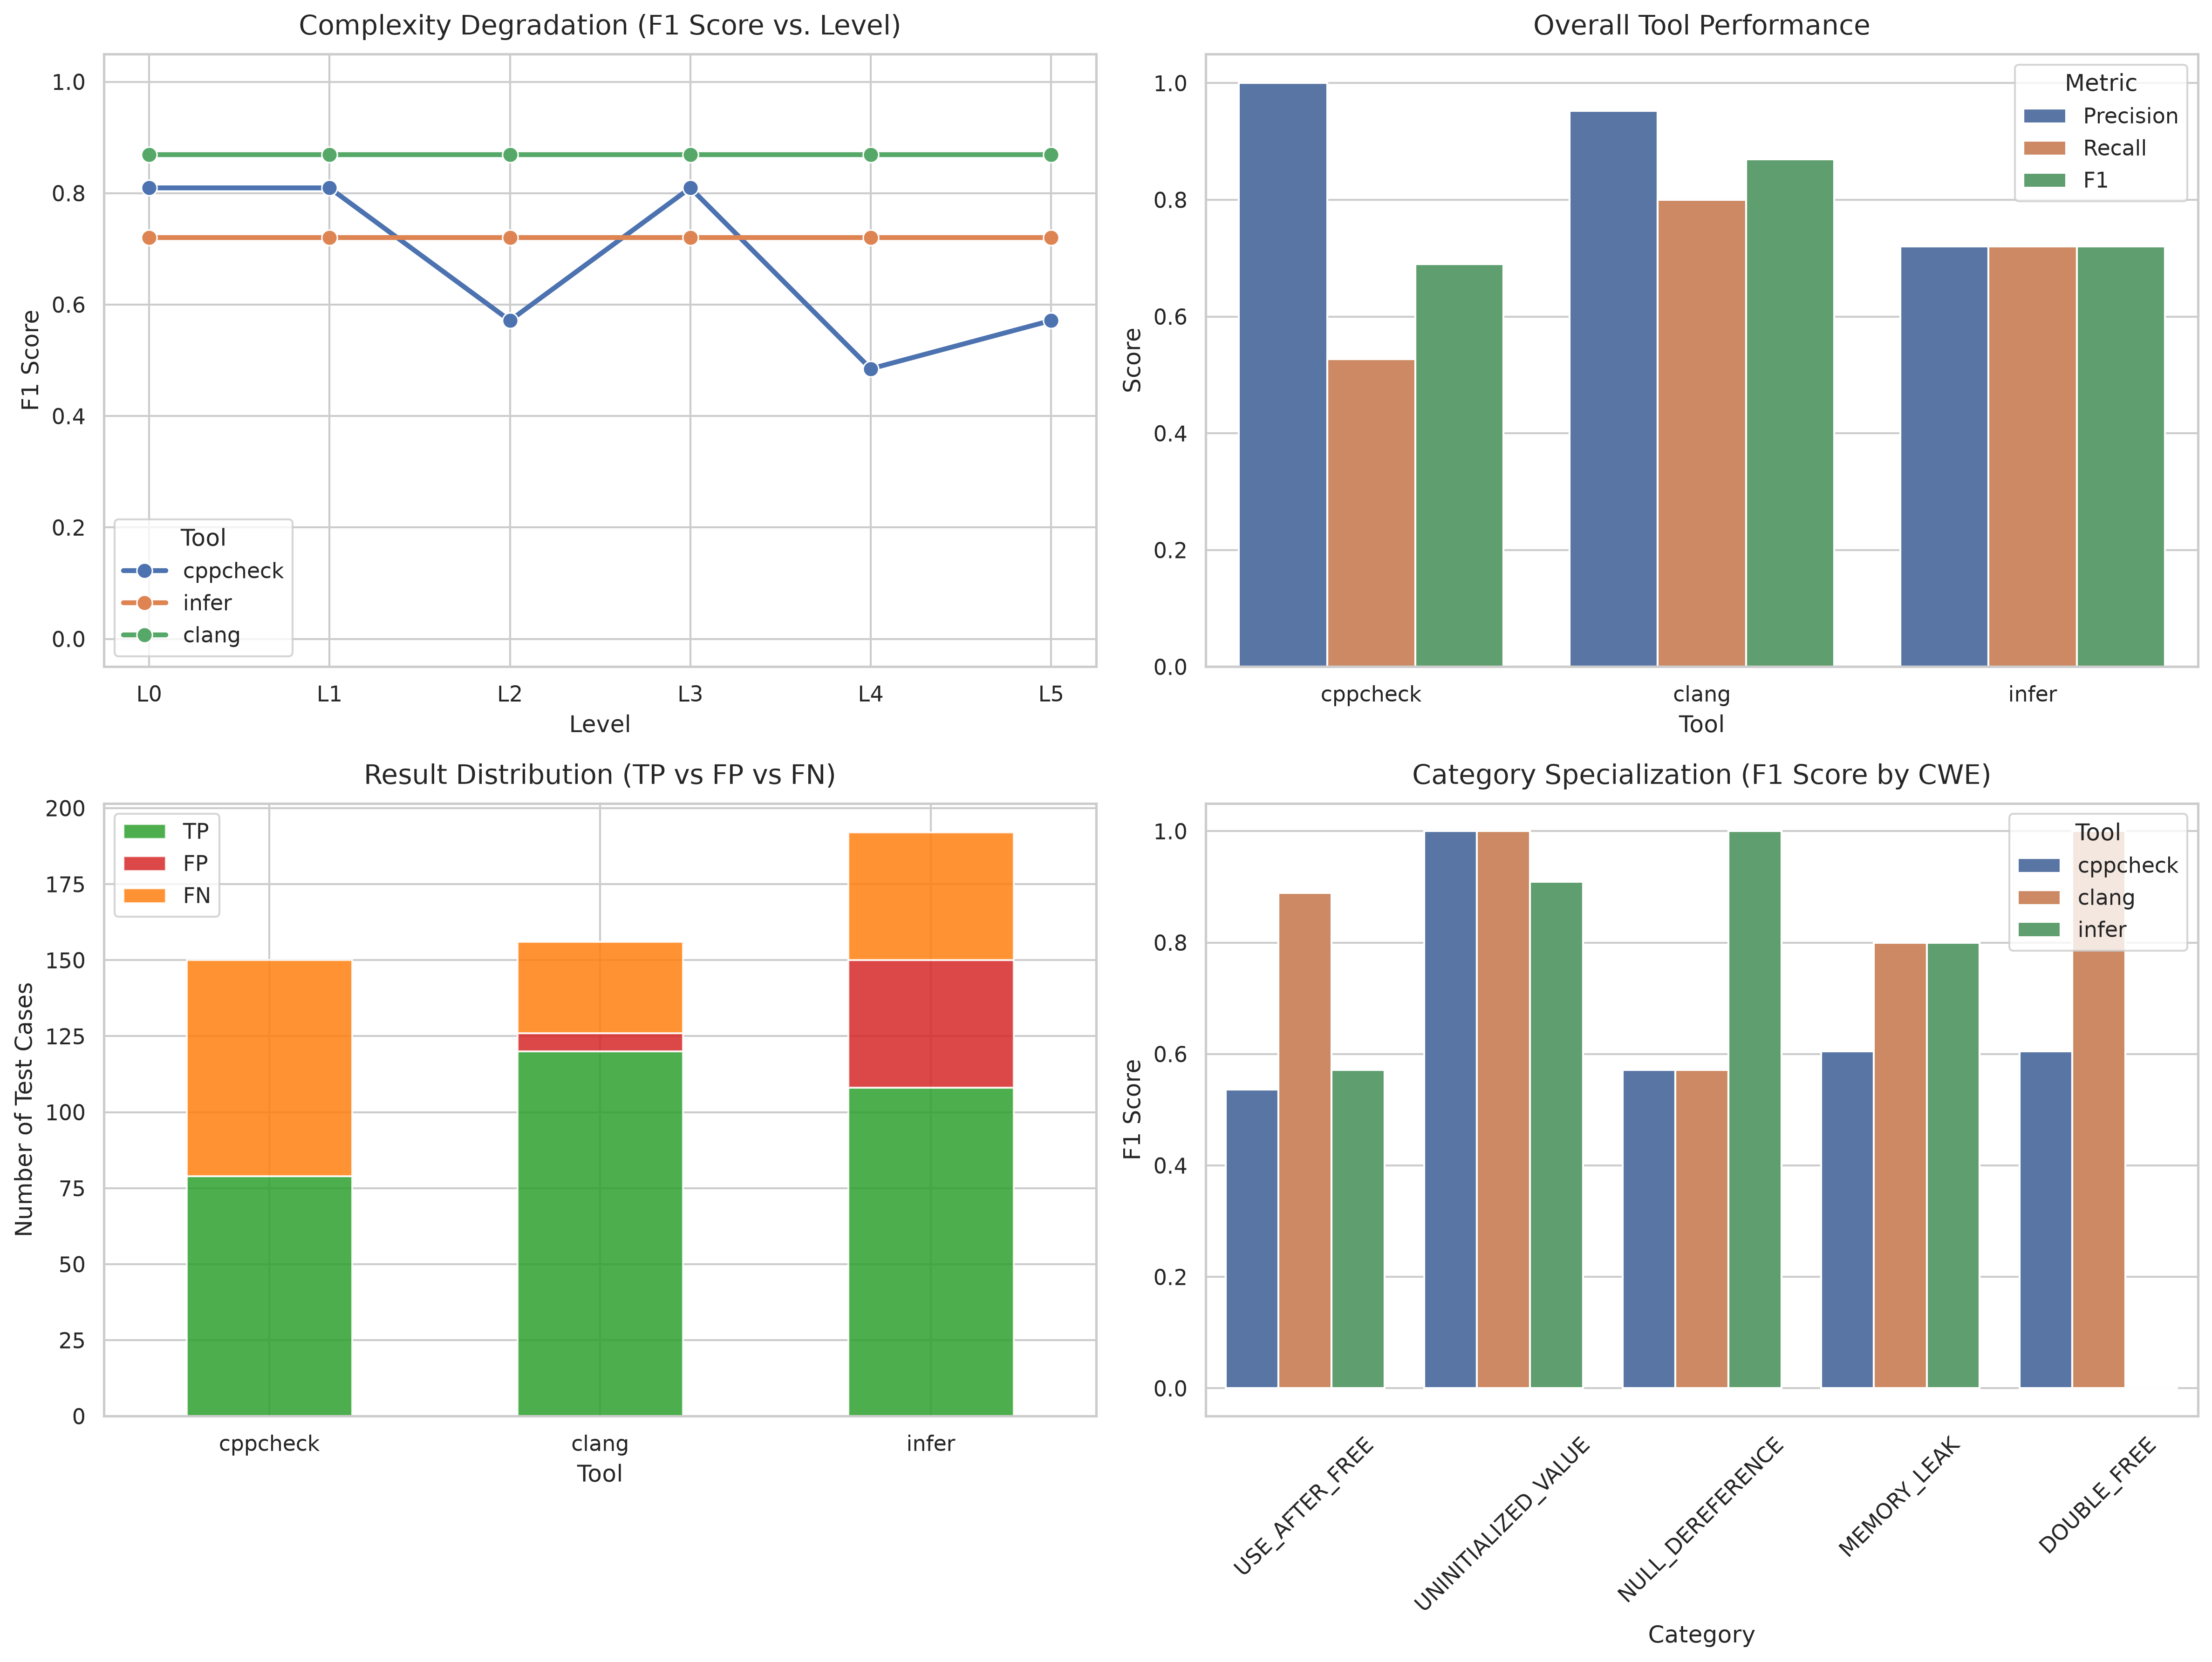
\includegraphics[width=\linewidth]{benchmark_results.png}
    \caption{Benchmark results of evaluated static analysis tools}
    \label{fig:grpah-results}
\end{figure}

\subsection{Overall performance}

Table~\ref{tab:overall_results} summarizes the aggregated results across all tested
vulnerability categories and complexity levels.

\begin{table}[ht]
\centering
\caption{Overall static analysis performance}
\begin{tabular}{lrrrrr}
\hline
Tool & TP & FP & FN & Precision & F1 \\
\hline
Clang & 120 & 6 & 30 & 0.952 & 0.870 \\
Cppcheck & 79 & 0 & 71 & 1.000 & 0.690 \\
Infer & 108 & 42 & 42 & 0.720 & 0.720 \\
\hline
\end{tabular}
\label{tab:overall_results}
\end{table}


Clang achieved the highest overall F1 score (0.870), providing the best balance
between detection capability and false positive rate. Cppcheck achieved perfect
precision, producing no false positives, but showed significantly lower recall due
to a higher number of missed vulnerabilities. Infer produced a balanced number of
false positives and false negatives, resulting in an F1 score of 0.720.


\subsection{Impact of code complexity}

The influence of source-code transformations is shown in Table~\ref{tab:complexity}.
The results indicate that Clang and Infer maintained stable detection performance
across all mutation levels.

\begin{table}[ht]
\centering
\caption{Effect of complexity levels on overall F1 score}
\begin{tabular}{lrrrrrr}
\hline
Tool & L0 & L1 & L2 & L3 & L4 & L5\\
\hline
Clang & 0.870 & 0.870 & 0.870 & 0.870 & 0.870 & 0.870\\
Infer & 0.800 & 0.800 & 0.800 & 0.800 & 0.800 & 0.800\\
Cppcheck & 0.810 & 0.810 & 0.571 & 0.810 & 0.485 & 0.571\\
\hline
\end{tabular}
\label{tab:complexity}
\end{table}


This suggests that the analysis engines used by Clang and Infer are robust against
the tested transformations, including interprocedural calls, aliasing, and additional
control-flow structures. In contrast, Cppcheck showed sensitivity to specific
transformations, especially those involving indirect memory access and additional
data-flow complexity.


\subsection{Category-level analysis}

Selected category-level results are presented in Table~\ref{tab:cwe_results}.

\begin{table}[ht]
\centering
\caption{Selected vulnerability category results}
\begin{tabular}{llrrr}
\hline
Tool & Category & Precision & Recall & F1\\
\hline
Clang & DOUBLE\_FREE & 1.000 & 1.000 & 1.000\\
Clang & NULL\_DEREFERENCE & 1.000 & 0.400 & 0.571\\
Clang & UNINITIALIZED\_VALUE & 1.000 & 1.000 & 1.000\\
\hline
Cppcheck & UNINITIALIZED\_VALUE & 1.000 & 1.000 & 1.000\\
\hline
Infer & NULL\_DEREFERENCE & 1.000 & 1.000 & 1.000\\
Infer & DOUBLE\_FREE & 0.000 & 0.000 & 0.000\\
\hline
\end{tabular}
\label{tab:cwe_results}
\end{table}


The category-level evaluation confirms that uninitialized value detection is a
well-supported analysis problem, with Clang and Cppcheck achieving perfect scores.
Infer performed particularly well on NULL pointer dereference detection. The lower
DOUBLE\_FREE score of Infer is influenced by category normalization, as related
memory errors may be reported under different analyzer-specific classifications.

\subsection{Conclusion}

This study evaluated three static analysis tools — Cppcheck, Clang Static Analyzer, and
Facebook Infer — across five memory-safety vulnerability categories and six levels of
source-code complexity generated by a purpose-built mutation framework.

The results demonstrate that the underlying analysis paradigm has a stronger influence
on detection behaviour than the specific vulnerability category. Clang's path-sensitive
symbolic execution achieved the best overall balance (F1 = 0.870), maintaining stable
detection across all complexity levels by tracking memory region state along individual
execution paths. Infer's compositional bi-abduction approach reached comparable
stability (F1 = 0.800 overall) and excelled on NULL pointer dereference detection
(F1 = 1.000), but its internal heap model caused double-free instances to be
reported as use-after-free, collapsing its measured DOUBLE\_FREE score to zero under
the fixed CWE-based evaluation scheme. Cppcheck's pattern-based, largely
intra-procedural checker achieved perfect precision (no false positives) but proved
sensitive to transformations that break its per-variable state machine, particularly
aliasing through struct fields (L2, F1 = 0.571) and loop wrapping (L4, F1 = 0.485).

The experiment confirms the theoretical prediction from Section~\ref{sec:background}:
tools that track state by variable name rather than by abstract heap address lose
coverage precisely when aliasing or inter-procedural boundaries are introduced, while
tools grounded in symbolic heap models or separation logic maintain coverage at the
cost of higher false-positive rates or category misclassification.

\subsection{Future Work}

The experiments showed that increasing source-code complexity through the
introduced mutation levels (L0--L5) did not significantly affect the detection
performance of Clang and Infer. Both tools maintained stable results despite
additional control-flow, interprocedural, and aliasing transformations.

Future work should evaluate these findings on a larger and more diverse
benchmark. The current manually created dataset could be extended with
established vulnerability collections such as the NIST Juliet Test Suite. The
existing mutation framework could then be applied to generate additional
complexity variants and further investigate tool robustness.

Additionally, testing on larger real-world C/C++ projects could provide a more
realistic evaluation of static analysis performance in complex software
environments.





\section*{Acknowledgments}

Generative AI tools, specifically OpenAI ChatGPT and Anthropic Claude Sonnet, were used for proofreading, language refinement, formatting suggestions, improvement of text clarity and for sanity check of the manually created tests cases.


\bibliographystyle{plain}
\bibliography{references}
	      
\end{document}